\chapter{Study of algorithms for containers allocation and load balancing}
\lhead{Chapter 5. \emph{Study of algorithms for containers allocation and load balancing}}
\label{chapt:containerloadbalance}

\section{Experimental applications}

The experimental process aims at measuring the performance of a set of
containers before and/or after using any resource allocation algorithm. First,
we have to define which applications will be containerized for those
operations. Those applications have to be deployed on all the agent servers and
have to behave as standard web services. Whatever is the language or the
framework used (except PHP), all the dependencies of the applications are
loaded on application startup, so afterwards, there is no more file to read
from the disk. It results in low input/output for most of the applications and
this metric will not be measured.

The first service which has been used during the experiments is an application which
is calculating $N$ elements of the Fibonacci suite\footnote{\textbf{Docker}
image: \texttt{soulou/msc-thesis-fibo-http-service}}. This web application has
only one endpoint: \texttt{GET /:n}, which returns the $N^{th}$ items, of the
Fibonacci sequence. This application only consumes CPU, the memory footprint is
really negligible.

The second application has been designed to consume a precise amount of
resource during a specified duration\footnote{\textbf{Docker} image:
\texttt{soulou/msc-thesis/memory-http-service}}. Its endpoint is \texttt{GET
/:memory/:time} with the memory in megabytes and the time in milliseconds. For
instance, \texttt{GET /10/100} will consume precisely 10MB for a duration of
0.1s. Thanks to this application, we can measure precisely how much should
consume the application with a load of $N$ requests per second of a certain
amount of memory during a precise timelapse.  The memory is allocated and
initialized. As a result, even if we are requesting amount of memory, it also
generates an important CPU load in the loops for memory application.

The source code of both services can be found on \textbf{GitHub}:
\begin{itemize}
\item{\url{https://github.com/Soulou/msc-thesis-fibo-http-service}}
\item{\url{https://github.com/Soulou/msc-thesis-memory-http-service}}
\end{itemize}

\section{Load generation}

An important question when measuring performance is the way to generate the
requests. Do they have to reflect a realistic user load, is it possible to do
it, is it pertinent? In this case, we are going to measure raw performance
over the cluster, to gather data about the efficiency of a specific algorithm.
When user load simulation algorithm is used, the benchmark is irregular, and
finally getting information about the real impact of a given algorithm may be
more difficult to do.

\subsection{Tools}

To generate web traffic, HTTP requests generators are required. Historically,
the most used tool is part of the \textbf{Apache} web server tools, and is
called Apache Bench \textit{Command line name: ab}, released under the
open-source \textit{Apache Licence}. This utility is not really used anymore
because it is single-threaded which. This is a very limiting caracteristic,
only one CPU core is used, it may not be enough to saturate a target and get a
correct measure of the performance.

The tool which has been mostly used in the scope of this work is named
\textbf{wrk}\footnote{\url{https://github.com/wg/wrk}}. This is a benchmark
tool able to send requests using a given number of connections, used in
different parallel threads. (The opposite of \texttt{ab}, which sends all
the request concurrently using one thread)

Usage example:

\vspace{1em}
\begin{lstlisting}
wrk -c 10 -t 2 -d 1m http://service1.thesis.dev
\end{lstlisting}

This example will send 10 requests concurrently during 1 minute using two threads.
So we are sure that the targeted URL will receive a maximum of 10 request at a
given time.

One reproach which can be made to this tool is that it doesn't adjust the
number of threads automatically. By default, two threads are used, but if we
need more parallel connections, the user has to define it by hand. But is most
of the case, giving a thread per core on the underlying computer is the
best practice.

\subsection{Different kinds of load}

Combining \textbf{wrk} and the two previously defined web application, different
kinds of load can be generated. Thanks to the "memory" HTTP service, it is even
possible to emulate different kinds of application.

\subsection{Lightweight services}

In some cases, web applications are micro-services and their job is to do a small
particular task. Commonly, requests are really quick and the treatment of each of
them has a low memory footprint. However as those HTTP requests may be numerous,
the overall processor and memory usage can be important.

In out infrastructure, one container of such a service may be represented by instances
of the memory services with requests using a few megabytes of memory, are done
really quickly: \texttt{http://micro-service.thesis.dev/5/100}. All the requests to this
endpoint are compliant with the previous constraints. The following data show how 
such application behave in an environment where they don't have to share resources\footnote{All the measure
have been done 5 times, and the given result is  the average}:

\begin{itemize}
	\item{One instance: \newline
	\texttt{wrk -c 20 `http://memory-service.thesis.dev/5/100'} --- 82.05req/s --- CPU 106\%, 24MB \newline
	\texttt{wrk -c 40 `http://memory-service.thesis.dev/5/100'} --- 93.74req/s --- CPU 112\%, 22MB \newline
	There is no big difference when running 20 or 40 connections in parallel, so we can assume that we have
	reached the maximum capacity of the instance. As announced previously, the memory usage is really low, but
	the application is using one complete core.\vspace{1em}}
	\item{Two instances on two different hosts: \newline
	\texttt{wrk -c 20 `http://memory-service.thesis.dev/5/100'} --- 123.23req/s --- CPU 109\% | 80\%, 15MB | 14MB \newline
	\texttt{wrk -c 40 `http://memory-service.thesis.dev/5/100'} --- 165.77req/s --- CPU 117\% | 97\%, 17MB | 31MB \newline
	The exepectations were that two instances would be able to execute twice the number of requests compared to
	the previous case. With 20 connections, it is not the case, but with 40, the service has been able to execute
	165 requests per second, which is more or less the double as previously. 20 connections was not enough. This
	lack can be seen by the fact that the CPU usage of one of the instances is not one complete core but 80\%.}
	\item{Two instances on the same host: \newline
	\texttt{wrk -c 20 `http://memory-service.thesis.dev/5/100'} --- 101.11req/s --- CPU 97\% | 98\%, 17MB | 18MB \newline
	\texttt{wrk -c 40 `http://memory-service.thesis.dev/5/100'} --- 127.77req/s --- CPU 115\% | 117\%, 18MB | 17MB \newline
	The instances have 2 vCPUs, so theoretically two instances of a same service on one node should be able to run
	at maximumal performance, but in practice, the results are not as good, a ratio of 1.5 has been reached using
	40 parallel connections. This is a perfect illustration of a ``bad neighbour'' situation, the performance of
	each container is jeopardized by the other instance. That is something which can be (at least partially) solved
	with scheduling algorithms, to avoid as much as possible this case.}
\end{itemize}

Note: The values of CPU usage are often above 100\% when an application is
using on core.  The amount of \textit{User HZ} is read every second, so it may
be an inacurracy of this timer, or it may be that the time used by the kernel
to schedule processes is taken into account. As a result, the process uses
100\% and the kernel uses some CPU time on another core.

\subsection{Bigger services}

The opposite of previous microservices are more important web services, consuming
more memory per request, with a lower number of request per second:

\begin{itemize}
	\item{One instance: \newline
	\texttt{wrk -c 20 `http://memory-service.thesis.dev/50/500'} --- 10.79req/s --- CPU 122\%, 326MB \newline
	\texttt{wrk -c 40 `http://memory-service.thesis.dev/50/500'} --- 9.30req/s --- CPU 116\%, 293MB \newline
	\vspace{1em}}
	\item{Two instances: \newline
	\texttt{wrk -c 20 `http://memory-service.thesis.dev/50/500'} --- 19.48req/s --- CPU 122\% | 80\%, 259MB | 182MB \newline
	\texttt{wrk -c 40 `http://memory-service.thesis.dev/50/500'} --- 23.26req/s --- CPU 102\% | 98\%, 302MB | 283MB \newline
	\vspace{1em}}
	\item{Two instances on one node: \newline
	\texttt{wrk -c 20 `http://memory-service.thesis.dev/50/500'} --- 19.48req/s --- CPU 109\% | 106\%, 153MB | 170MB \newline
	\texttt{wrk -c 40 `http://memory-service.thesis.dev/50/500'} --- 19.43req/s --- CPU 105\% | 101\%, 202MB | 195MB \newline
	\vspace{1em}}
\end{itemize}

Except the fact he the servers suppor less requests as each of them is heavier,
the behaviour between a light application and this one is prett similar. It
scales out correctly, doubling the mount of requests the service can manage.
With this application even if the memory consumption is getting higher, the
limiting resource is still the processor. The fact that the CPU is in most of
the case the resource causing a bottleneck is something
common.~\cite{reassignmentElectricitysaving, reassignmentVisbp}

In the previous examples we have done performance benchmark, the maximum
performance of the services have been measured. But with \textbf{wrk}, it
is possible to send a lower amount of requests to simulate a normal load.
When 1 to 10 connections are used (instead of 20 or 40) like in the previous
experiment, the resulting CPU consumption would vary respectively 
between 10 and 100\%

\section{Bin packing algorithms}

Bin packing algorithms have been defined in the~\cref{litreview}, but here is a
short reminder about the main ideas behind them.  A bin packing algorithms
consist in packing items into bins. Each bin has a capacity and each item
weighs certain size. There are two main categories: online bin packing and
offline bin packing. The first type is defined by the following setup. The bins
are already filled with items, but we can't have details about those items.
There is a new item to pack, the online bin packing algorithms have to choose
the best bin for the new item.  The offline bin packing algorithms consider
that all the bins are empty, and it has to pack all the items into the bins.
All the information about each item is available.

We speak of bin packing algorithms with the plural, because there isn't only
one way to pack items, offline bin packing is an NP-Hard problem, finding the
optimal solution can be very long. That's why a large number of heuristics
exist to get a good enough result in a short enough period.

\subsection{Relation with resource allocation}

In our situations, the items are the appications containers and the bins are
the different hosts, here OpenStack virtual machines. Different operations
can be done when packing application containers:

\begin{itemize}
	\item{Consolidation: Use the minimum of hosts to run correctly all the containers}
	\item{Load balancing: Balance the load over the available hosts}
	\item{Container Allocation: Choice of the best node to run a new container}
\end{itemize}

First, it is important to define the fact that the resource consumption of a
container is completely ephemeral. As the resources are not completely
dedicated to a container, but shared with each other, the container may have
to be moved soon after its allocation, when its load has been defined. That's
why using only resource allocation is not enough to balance correctly the
infrastructure.

As the consumption of CPU is variable, it is important to keep a security
reserve. If the amount of requests to a container increases, it has to be
able to get more CPU time, otherwise it will the stucked and all the requests
would be impacted. That's why, there is a default margin of 20\% in the
platform we are using. It means that if a server is loaded up to 50\% and
that a new container estimated at 40\% has to be packed. The server wouldn't
be considered as available as the total is over 80\% (for a one core server)

\subsection{Container allocation --- online bin packing algorithms}

\subsubsection{Type of new items}

Online bin packing means that we have to pack new items into bins without
having the knowledge of what is already present in the bins. So bins have a
remaining capacity, and each new items is known or partially known. In some
cases, the new items are completely unknown.

In this infrastructure there are two different cases which can be distinguished:

\begin{itemize}
\item{The new container is part of a new service: there is no information about
the number of incoming requests, and what is the memory footprint of the new process}
\item{The new container is from an existing service: in this case, the CPU consumption
and memory usage can be estimated by looking the other containers of a similar service.
For instance, if two containers of \texttt{service1} are running using both 20\% of CPU,
it is probably true that the consumption of the new container will be capped at 20\%}
\end{itemize}

\subsubsection{Algorithms and Heuristics}

In the following part, different algorithms are going to be used. Some dummy
methods will be used as comparative methods. They are `random' and
`round-robin'. With those strategies, no bin packing is executed, the choice
of the server is determined randomly or through a round-robin loop.

Three basic algorithms of bin packing are used:

\begin{itemize}
	\item{First Fit: The item is packed on the first bin which is able to contain it}
	\item{Best Fit: The bin which is able to contain the item with the smallest capacity}
	\item{Worst Fit: The bin which is able to container the item with the biggest capacity}
\end{itemize}

Our nodes and containers are monitored over three metrics: ``CPU usage'',
``Memory usage'', ``Network I/O''.  As it has been shown previously, the only
resource wich is a bottleneck from far the the CPU\@. As a result the
algorithms have been implemented the following manner: when the item is
inspected to see if it can fit on one node, all the metrics are compared, if
one of them is insufficient, the allocation on this node is rejected. However
in best fit and worst fit, when we need to select the best, or the worst, only
the CPU is considered.

\subsubsection{Experiment - Comparaison of algorithms}

This experiment consists in starting a set of containers using different
algorithms to choose the destination node. There are 8 virtual machines with 2
cores, 7 of them are agents running the container and one is controller and
load balancer to route the HTTP requests to the instances. The containers are
splitted into 3 services of various sizes:

\vspace{1em}
\begin{tabular}{l | c | c | c | c}
	& Number of containers & Memory Usage & Request Duration & Parallel connections \\
	Service 1 & 4 & 10MB & 10ms & 30 \\
	Service 2 & 4 & 25MB & 200ms & 20 \\
	Service 3 & 2 & 50MB & 300ms & 10 \\
\end{tabular}
\label{tab:exp2-services}
\captionof{table}{Description of the experimental HTTP services}
\vspace{1em}

A container has been launched every 5 seconds to let the time to the monitoring
system to take it into account and to be able to measure its usage. The HTTP
requests are sent even before the first container has been created, be cause the
front-end server \textbf{Hipache} will drop the request answering the HTTP error
\textit{502 bad gateway}. As soon as a container from the given service is available
the requests are correctly routed to it.

The metric which is measured is the one important from an user perspective. The
number of requests answered per second. We are expecting worst-fit, random and
round-robin to get better results that first-fit and best-fit because they
don't try to optimize the number of used servers, but they will spread the services
on all of them.

For each algorithm, 5 executions have been done and the displayed value is the average
of the the result of each of the tries. One execution lasts 2 minutes, and the obtained
value is the amount of requests answered per second.

\begin{figure}[h!]
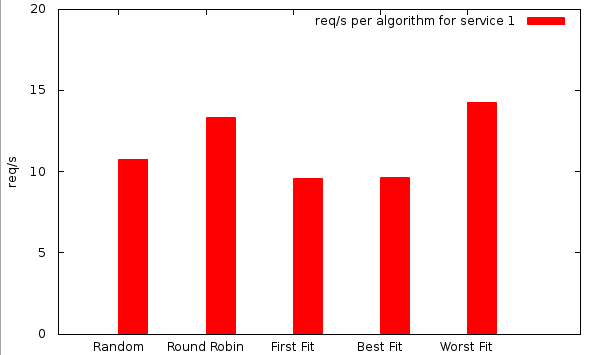
\includegraphics[width=\textwidth]{./Images/BinPacking/exp2-service1.png}
\label{fig:exp2service1}
\caption{Service 1: Number of requests per second for various algorithms}
\end{figure}

\begin{figure}[h!]
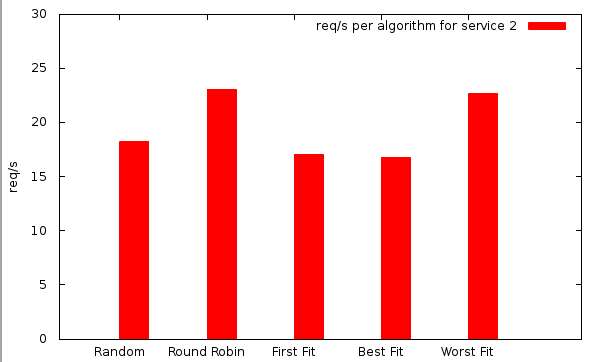
\includegraphics[width=\textwidth]{./Images/BinPacking/exp2-service2.png}
\label{fig:exp2service2}
\caption{Service 2: Number of requests per second for various algorithms}
\end{figure}

\begin{figure}[h!]
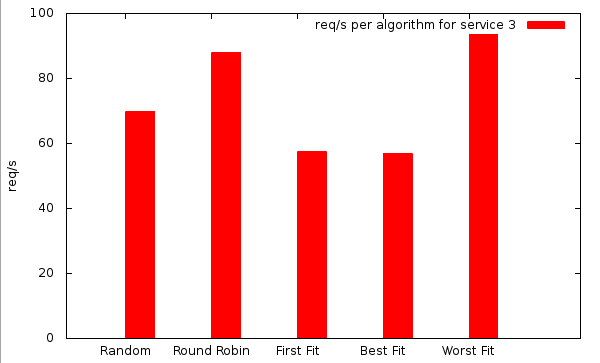
\includegraphics[width=\textwidth]{./Images/BinPacking/exp2-service3.png}
\label{fig:exp2service3}
\caption{Service 3: Number of requests per second for various algorithms}
\end{figure}

\vspace{1em}
\begin{tabular}{c | c | c | c}
	Algorithm & Number of used nodes & Performance rank \\
	Random & 7 & 3 \\
	Round-Robin & 7 & 2 \\
	First-Fit & 4 or 5 & 4 \\
	Best-Fit & 3 or 4 & 5 \\
	Worst-Fit & 7 & 1 \\
\end{tabular}
\captionof{table}{VMs allocation summary}
\vspace{1em}

\subsubsection{Results and discussions}

A first remark about those results is that, whatever is the service, and the
amount of requests it has to deal with, they behave the same way for each
algorithm. The graphs have the same shape with another ratio because some
container deal with much more queries.

Then, we can observe that as expected the best-fit and first-fit algorithms are
resulting to poorer performance. But what is shown in the allocation summary is
that those algorithms managed to use less virtual machines to pack all the
processes. They allocate resources on less than 5 of the 7 availables nodes.

Here is one of the biggest challenge, to get close to the highest performance
while using the minimum number of bins. There is direct solution for this problem
it really depends what is the main goal of the operation. If it is money saving,
reducing the number of virtual machines has a meaning, but the quality of service,
as the performance, should be high enough to respect the SLA\@.

Something which is more surprising is that an algorithm considered as
``intelligent'', which is worst fit, is only doing slightly better, and
sometimes even worse, than a simple algorithm like round robin.

The different *-fit algorithms need an estimation of the size of the incoming
item to pack. As stated previously, if the containers is part of an existing
service, the average of the usage of the other containers of this service will be
used. Otherwise, no estimation is done. This second condition seems to damage
those algorithm results.

To get over it, Some hybrid *-fit algorithms have been tried:

\begin{itemize}
	\item{Best-Worst Fit: This algorithm is using best-fit all the time except when
	the new item is from a new service, in this case, worst fit is used to pack
	it}
	\item{First-Worst Fit: Similar to best-worst fit but using first fit instead of 
	best-fit}
\end{itemize}

These variants should allocate more VMs than the base algorithms they are based on,
but they should be much more efficient for the same reason. As we have seen that the
results are mostly identical for the three differents services, we will focus on the
third one, it is not worthy to study the three of them.

\begin{figure}[h!]
	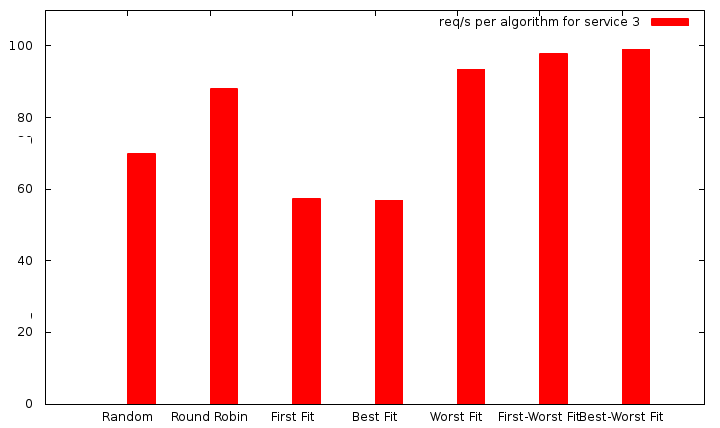
\includegraphics[width=\textwidth]{./Images/BinPacking/exp2ext-service3.png}
	\caption{Comparaison of *-fit algorithms performance}
\end{figure}

\vspace{1em}
\begin{tabular}{c | c | c | c}
	Algorithm & Number of used nodes & req/s for service 3 & Performance rank \\
	First-Worst Fit & 6 or 7 & 97.80 & 2 \\
	Best-Worst Fit & 5 or 6 & 99.05 & 1 \\
	Worst-Fit & 7 & 93.41 & 3 \\
\end{tabular}
\captionof{table}{Allocation summary with variants of *-fit algorithms}
\vspace{1em}

With these new results, we have successded to get slightly better results than
the standard worst-fit, and highly superior than the base algorithm each of the
variant is based on. First-Worst Fit and Best-Worst Fit are getting more or
less the same results but they are not using the same amount of nodes. From
that point, best-worst is clearly the best algorithm among them.  We could
alter those algorithms with some additional steps like sorting the bins before
starting the pack operation like it has been done
in~\cite{allocationHeterogeneous}.  However in this precise case it would be
without any effect. First-fit with ascending sorted bins result in Best-fit and
when the sort is descending it leads to Worst-fit, and we already know the
results of these methods.

We have seen that different methods exist, but to get a good ratio
performance/node usage, it may be required to mix the algorithms according to
the situation and the execution environment.  In our case, a mix of Best-fit
and Worst-fit has definitely got the most interessant results.

\subsection{Consolidation and load balancing --- offline bin packing algorithms}

\subsubsection{Impact on the infrastructure}

When an offline bin packing algorithm is applied on computing infrastructure,
to apply the new configuration, it results in a lot of migrations. When we are
dealing with full virtual machines, a migration has a cost and it is difficult
to imagine migrating several instances from one same host in parallel. With
containers, this issue doesn't exist and even less with stateless application

When a container has to be migrated, a new one is being started on the
destination server, then the routing table to the service is updated and
finally the source container is stopped. This operation can be done in less
than a second. Compared to VM migration which can last minutes and use a lot of
disk, network and CPU resources, the process which is used here costs almost
nothing.

If migrations were costly, caution should be taken when choosing the algorithm,
to avoid to do too many of them.

\subsubsection{Algorithms}

In this case, testing simple algorithms like round-robin or random would not be
interesting. They would result in the same data as what we have seen in the part
about online bin packing.

Offline bin packing algorithms are close to the online bin packing algorithm,
the differences are that we have all the pieces of information about the
running containers so there is no need to estimate any value. Then, there is
not only one item to pack anymore, but a list of items. An additional question
is in which order do the items have to be considered by the algorithms.
In~\cite{reassignmentElectricitysaving},~\cite{statisticalAssignment}
and~\cite{variableSizeBinPacking} they all refer to first-fit decreasing or
best-fit decreasing as reference algorithms. It means that the data are used
from the biggest to the smallest.

As a result 4 algorithms will be tested: Best-Fit Decreasing (BFD), First-Fit
Decreasing (FFD), the algorithm proposed by Michaël Gabay
in~\cite{variableSizeBinPacking} and the variant detailed
in~\cite{allocationHeterogeneous} where items are sorted decreasingly.

The used parameters are the following:

\begin{verbatim}
Gabay: heuristic=bin_balancing
Gabay: heuristic=bfd_item_centric
Gabay: heuristic=bfd_bin_centric
Stillwell: item_sort=d:maximal, pack=pack_by_items
\end{verbatim}

\subsubsection{Experiment}

The following experiment is based on the same services as the previous
experiment. This choice has been made because they have already been
benchmarked, and their range of performance is already known.  Refer to
the~\tref{tab:exp2-services}.

To obtain the data of the following graph, the underneath experiment has been done 5
times for each algorithm:

\begin{enumerate}
	\item{Start the load generation against the three services}
	\item{Deploy containers using a resource allocation algorithm which is not
	optimal. Best-fit has ben chosen because of the low result it has given in
	the previous experiment. This situation leads to overloaded nodes}
	\item{Run a first benchmark to get the performance before the offline bin
	packing algorithm execution}
	\item{Balance the infrastructure with the chosen algorithm}
	\item{Run a second benchmark to get the performance after the operation}
	\item{Calculate the average of the performance variation for the three services}
\end{enumerate}

Then once the previous protocol has been done 5 times, the average of the
result is the value displayed on the plot.\footnote{The detailed results for
the experiment can be found here:
\url{https://github.com/Soulou/msc-thesis-container-balancer-client/tree/master/experiment4}}

\begin{figure}[h!]
	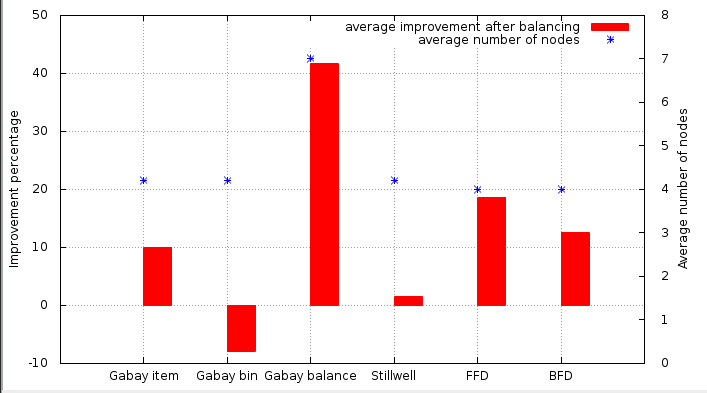
\includegraphics[width=\textwidth]{./Images/BinPacking/exp4_improvement.png}
	\caption{Performance improvement in function of the algorithm}
\end{figure}

\subsubsection{Results and Discussions}

The results are quite surprising. If \textit{Gabay balance} is shelved, the
different results are using the same amount of nodes, but their result are
unexpected.~\cite{allocationHeterogeneous} and~\cite{variableSizeBinPacking}
based their work on BFD and FFD, and build variations of them to fit specific
need, which is to work in an heterogeneous environment. Obviously it was not
the case here, but we could expect that those algorithms would have done at
least as good as BFD or FFD\@.

It is also possible that this error is due to a bad integration of the
algorithm in the container platform. Extensive testing would be required to
find if the behavior is buggy. It may be linked to how the data are normalized.
Everything is based on the bins. The server which as the highest capacity
results in the unit bin, with $1$ as capacity for each of his metrics, then all
the containers consumptions (items) and other bins are normalized using this
reference.  After this step, a reserve is subtracted from the capacity, to
avoid the algorithms to pack servers up to 100\% again. By default this reserve
is 20\%, and it seemd it suits well the implementations of BFD and FFD\@. But
Gabay's and Stillwell's algorithm are not working as they should. According to
their estimation in their work, they should both be more performant than BFD
and FFD\@.

The heuristic \textit{Gabay Balance} got great results which are really closed
to a simple worst fit allocation, all the nodes have been used and no effort
has been done to limit that. But, as a results, great performance is present.
If the goal of the operation is to balanced the load of the server, this approach
is probably the most efficient.

Comparing the two basics algorithms, FFD got slightly better results than BFD,
the difference is higher than the difference of those algorithms for online bin
packing, but the trend is similar. 

\vspace{1em}

Finally, the platform has proven that it is possible to get interesting metric
from it. In the previous experiments, containers have been deployed and
migrated with success resulting in performance variations. The three main
operation linked to resource allocation/re-assignment can be tested using this
infrastructure. If the online bin packing results are interesting, the data
collected for offline be packing are not resulting to a spcific recommandation.
